\documentclass[10pt]{book}
\usepackage[utf8]{inputenc}
\usepackage[italian]{babel}
\usepackage{multicol}
\usepackage[bookmarks]{hyperref}
\usepackage[a4paper, total={18cm, 25cm}]{geometry}
\usepackage{listings}
\usepackage{graphicx}
\usepackage{makecell}
\graphicspath{ {./img/} }
\usepackage{color}

\begin{document}
\renewcommand*\contentsname{Indice}
\title{Basi di Dati}
\author{Federico Matteoni}
\date{A.A. 2019/20}
\maketitle
\tableofcontents
\pagebreak
\chapter{Introduzione}
\paragraph{Obiettivi del corso} Modelli dei dati, linguaggi e sistemi per lo sviluppo di applicazioni che prevedono l'uso di grandi quantità di dati permanenti organizzati in \textbf{basi di dati}.
\paragraph{Testo di Riferimento} \textit{Fondamenti di Basi di Dati}, A. Albano, G. Ghelli e R. Orsini, Zanichelli. Scaricabile liberamente da \texttt{fondamentidibasididati.it}
\paragraph{Esame} Scritto $+$ orale
\paragraph{Terminologia}
\begin{list}{}{}
	\item \textbf{Base di dati}: tecnologia di base, gestione delle attività quotidiane dell'organizzazione e \textbf{tema di questo corso}
	\item Data Warehouse, Data Lake, Big Data, Data Science: termini che hanno a che vedere con l'\textbf{analisi dei dati} e che non rientrano nei temi trattati nel corso.
\end{list}
\chapter{Base di Dati}
\paragraph{Cos'è una base di dati?} Una \textbf{base di dati} è un \textbf{insieme organizzato di dati} usati per il supporto allo svolgimento di una attività (di un ente, azienda, ufficio, persona\ldots)
\paragraph{Qualche esempio}
\begin{center}
\textbf{Materie}\\
	\begin{tabular}{c | c | c}
	\textbf{Titolo} & \textbf{Codice} & \textbf{Syllabus} \\
	\hline
	Basi di Dati & AA024 & Progettazione e interrogazione\ldots \\
	\hline
	Reti di Calcolatori & AA019 & Realizzazione e uso di reti, protocollo TCP\ldots
	\end{tabular}
\end{center}
\begin{center}
\textbf{Corsi}\\
	\begin{tabular}{c | c | c | c}
	\textbf{Materia} & \textbf{AA} & \textbf{Semestre} & \textbf{Titolare} \\
	\hline
	AA024 & 2007 & 1 & Albano \\
	\hline
	AA024 & 2007 & 1 & Ghelli \\
	\hline
	AA019 & 2007 & 1 & Brogi 
	\end{tabular}
\end{center}
\section{Costruzione di una Base di Dati}
\subsection{Figure Coinvolte}
\begin{list}{}{}
	\item \textbf{Committente}
	\begin{list}{}{}
		\item Dirigente
		\item Operatore
	\end{list}
	\item \textbf{Fornitore}
	\begin{list}{}{}
		\item Direttore del progetto
		\item Analista
		\item Progettista del DB
		\item Programmatore di applicazioni che usano il DB
	\end{list}
	\item Manutenzione e messa a punto del DB -- Gestione del DBMS
	\begin{list}{}{}
		\item Amministratore del DBMS
	\end{list}
\end{list}
\subsection{Sistemi Informativi}
\paragraph{Definizione} Un \textbf{sistema informativo} di un'organizzazione è una \textbf{combinazione di risorse, umane e materiali, e di procedure} organizzate per raccolta, archiviazione, elaborazione e scambio \textbf{delle informazioni} necessarie alle attività:
\begin{list}{}{}
	\item Operative (informazioni di servizio)
	\item Programmazione e controllo (informazioni di gestione)
	\item Pianificazione strategica (informazioni di governo)
\end{list}
\pagebreak
\paragraph{Esempi di sistemi informativi}
\begin{list}{}{Un comune}
	\item Gestione servizi demografici (anagrafe, stato civile, servizio elettorale e vaccinale) e della rete viaria
	\item Gestione attività finanziaria secondo la normativa vigente
	\item Gestione del personale per il calcolo della retribuzione in base al tipo di normativa contrattuale
	\item Gestione dei servizi amministrativi e sanitari delle USL
	\item Gestione della cartografia generale e tematica del territorio
\end{list}
\paragraph{Sistema informativo nelle organizzazioni}
\begin{center}
	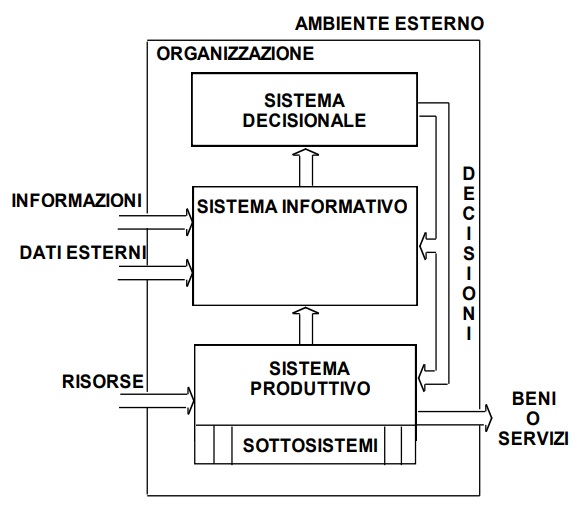
\includegraphics[scale=0.7]{sisinformativoorg.png}
\end{center}
\subsection{Sistemi Informatici}
\paragraph{Sistema Informativo Automatizzato} Quella parte del sistema informativo in cui le informazioni sono raccolte, elaborate, archiviate e scambiate usando un \textbf{sistema informatico}.
\paragraph{Sistema Informatico} Insieme delle tecnologie informatiche e della comunicazione (\textbf{ICT}, Information and Communication Technologies) a supporto delle attività di un'organizzazione.
\paragraph{Terminologia}
\begin{center}
Sistema informativo $\longrightarrow$ Sistema informativo automatizzato\\
Sistema informativo automatizzato $\longrightarrow$ Sistema informatico
\end{center}
\begin{center}
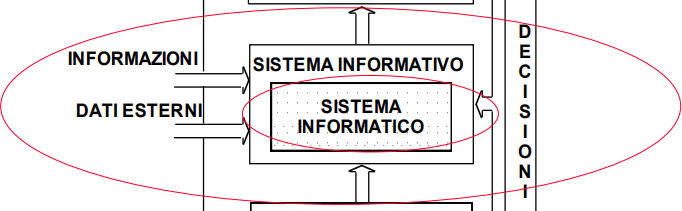
\includegraphics[scale=0.7]{sisinformativoorg2.png}
\end{center}
\pagebreak
\subsection{Classificazione dei sistemi informatici}
\begin{center}
Sistemi Informatici Operativi $\longrightarrow$ Sistemi Informatici Direzionali
\end{center}
\begin{multicols}{2}
\paragraph{Sistemi Informatici Operativi} I dati sono organizzati di DB. Le applicazioni si usano per svolgere le classiche attività strutturate e ripetitive dell'azione nelle aree amministrativa e finanziaria: vendite, risorse umane, produzione\ldots\\
\textbf{Alcune sigle}:
\begin{list}{}{}
	\item \textbf{DP} Data Processing\\\textbf{EDP} Electronic Data Processing
	\item \textbf{TPS} Transaction Processing Systems
\end{list}
\begin{center}
	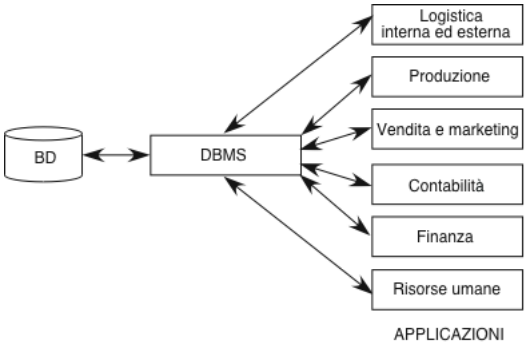
\includegraphics[scale=0.6]{sisinfop.png}
\end{center}
\paragraph{DBMS} Le caratteristiche del DB sono \textbf{garantite da un sistema per la gestione della base di dati} (\textbf{DBMS}, Data Base Management System) che ha il controllo dei dati e li rende accessibili agli utenti autorizzati.
\paragraph{OLTP} \textbf{On-Line Transaction Processing}, modo d'uso principale dei DBMS. Tradizionale elaborazione di transazioni, che realizzano processi operativi per il funzionamento di organizzazioni:
\begin{list}{}{}
	\item Operazioni predefinite e relativamente semplici
	\item Ogni operazione coinvolge \textit{pochi} dati
	\item Dati di dettaglio, aggiornati
\end{list}
\end{multicols}
\begin{multicols}{2}
\paragraph{Sistemi Informatici Direzionali} I dati sono organizzati in data warehouse (DW) e gestiti ad un opportuno sistema. Le applicazioni, dette di \textbf{business intelligence}, sono strumenti di supporto ai processi di controllo delle prestazioni aziendali e di decisione manageriale. Terminologia:
\begin{list}{}{}
	\item \textbf{MIS} Management Information Systems
	\item \textbf{DSS} Decision Support Systems, data-based o model-based
	\item \textbf{EIS} Executive Information System
\end{list}
\begin{center}
	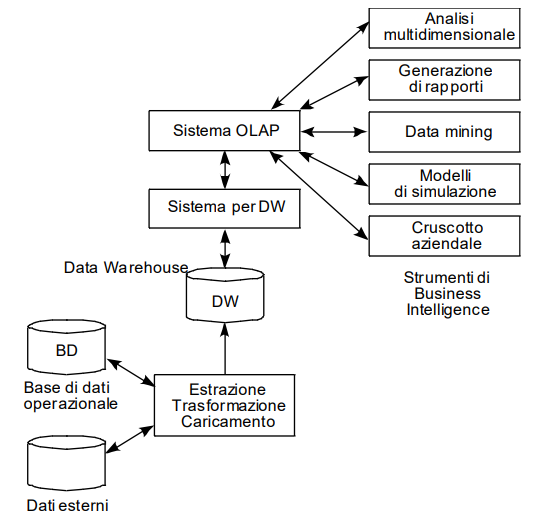
\includegraphics[scale=0.6]{sisinfdir.png}
\end{center}
\columnbreak
\paragraph{OLAP} \textbf{On-Line Analytical Processing} modo d'uso principale dei DW. Analisi dei dati di supporto alle decisioni:
\begin{list}{}{}
	\item Operazioni complesse e casuali
	\item Ogni operazione può coinvolgere \textit{molti} dati
	\item Dati aggregati, storici, anche non attualissimi
\end{list}
\end{multicols}
\pagebreak
\paragraph{Differenze tra OLTP e OLAP}
\begin{center}
	\begin{tabular}{c | p{5 cm} | p{5 cm}}
	 & \makecell{\textbf{OLTP}} & \makecell{\textbf{OLAP}} \\
	\textbf{Scopi} & Supporto operatività & Supporto decisioni \\
	\textbf{Utenti} & Molti, esecutivi & Pochi, dirigenti e analisti \\
	\textbf{Dati} & Analitici, relazionali & Sintetici, multidimensionali \\
	\textbf{Usi} & Noti a priori & Poco prevedibili \\
	\textbf{Quantità di dati per attività} & Bassa (decine) & Alta (milioni) \\
	\textbf{Orientamento} & Applicazione & Soggetto \\
	\textbf{Aggiornamenti} & Frequenti & Rari \\
	\textbf{Visione dei dati} & Corrente & Storica \\
	\textbf{Ottimizzati per} & Transazioni & Analisi
	\end{tabular}
\end{center}
\subsection{Requisiti per l'Analisi dei Dati}
\paragraph{Aggregati} Non interessa \textbf{un} dato, ma la \textbf{somma}, la \textbf{media}, il \textbf{minimo}/\textbf{massimo} di una misura\ldots
\paragraph{Multidimensionale} Interessa \textbf{incrociare le informazioni}, per analizzarle da punti di vista diversi e valutare i risultati del business per intervenire sui problemi critici o per cogliere nuove opportunità
\paragraph{Diversi livelli di dettaglio} Per esempio, una volta scoperto un calo delle vendite in un determinato periodo in una specifica regione, si passa ad un'analisi dettagliata nell'area di interesse per cercare di scoprirne le cause (dimensioni con \textbf{gerarchie})
\subsection{Big Data}
\paragraph{Ampio} Big data è un termine ampio riferito a situazioni in cui l'approccio "schema-first" tipico di DB e DW risulta troppo restrittivo o troppo lento.
\paragraph{3 V} Volume, Varietà, Velocità
\paragraph{} I Big Data sono in genere associati a sistemi NoSQL, machine learning e approcci Data Lake.
\end{document}